\documentclass[11pt]{article}
\usepackage{amsmath,amssymb,amsthm}
\usepackage{graphicx}
\usepackage[margin=1in]{geometry}
\usepackage{fancyhdr}
\setlength{\parindent}{0pt}
\setlength{\parskip}{5pt plus 1pt}
\setlength{\headheight}{13.6pt}
\newcommand\question[2]{\vspace{.25in}\hrule\textbf{#1: #2}\vspace{.5em}\hrule\vspace{.10in}}
\renewcommand\part[1]{\vspace{.10in}\textbf{(#1)}}
\newcommand\algorithm{\vspace{.10in}\textbf{Algorithm: }}
\newcommand\correctness{\vspace{.10in}\textbf{Correctness: }}
\newcommand\runtime{\vspace{.10in}\textbf{Running time: }}
\pagestyle{fancyplain}
\lhead{\textbf{\NAME\ (\ANDREWID)}}
\rhead{Page \thepage}
\begin{document}\raggedright


%Section A==============Change the values below to match your information==================
\newcommand\NAME{Turaga}  % your name
\newcommand\ANDREWID{nturaga1@jhmi.edu}     % your andrew id
%\newcommand\HWNUM{1}              % the homework number

\title{Shyam Biswal : MeDIP on 2.1M Nimblegen Array}
\author{Nitesh Turaga}
\maketitle
%%%%%%%%%%%%%%%%%%%%%%%%%%
\section*{Analysis}
%%%%%%%%%%%%%%%%%%%%%%%%%%

Data from Shyam Biswal, used to compare the differential methylation regions of H460 Knocking cell line and H460 parent cell line.

%%%%%%%%%%%%%%%%%%%%%%%%%%
\section*{Data Description}
%%%%%%%%%%%%%%%%%%%%%%%%%%

Data was generated from two color Nimblegen microarrays. The raw Nimblegen data was in the form of {\tt .tif} images and the corresponding array design files were given for building the annotation package {\tt 100929\_HG19\_Deluxe\_Prom\_Meth\_HX1}  with {\tt pdInfoBuilder}.

Array images were processed with DEVA-v1.2 (Nimblegen software for automated feature extraction and data analysis). The TIF files were processed and converted to {\tt .xys} files for analysis. The TIF files were also processed with DEVA using the DNA methylation work flow to identify peaks and generate a result for each sample.


%%%%%%%%%%%%%%%%%%%%%%%%%% 
\section*{Preliminary Assessments}
%%%%%%%%%%%%%%%%%%%%%%%%%%

{\bf Analysis using CHARM}

Initial array quality assessment was done using {\tt charm} and the {\tt .xys} files. 

Array quality scores were generated with {\tt charm::qcReport}, and data quality was checked using the $Enriched$ channel. Four of the six arrays show a large standard deviation in the signal strenth and seem to have a problem in hybridization. {\tt charm::pmQuality}, provides the array signal quality score. 3 of the samples have a signal strength above the cutoff(70).

{\tt Refer: qcReport.pdf}


Charm fails to find DMR’s both while taking into account surrogate variables(SV) and not while not accounting for SV's. This might be because the image quality is poor after hybridization with a lot of variability in 3 out of the 6 images. The case control being used is the “H460\_parent” vs “H460\_knockin”. No other annotation is recorded in the experimental metrics {\tt .xlsx} file given.



{\bf Analysis using Bumphunter}

\begin{enumerate}

\item Run  1

Initially ran {\tt bumphunter} on the data, with cutoff value 1.0, this failed to find any bumps. The sensitivity of the cutoff was not enough to catch any DMRs in the sample set. Bumphunter is better used for large sample sets, for better performance. 


\item Run  2

Bumphunter, with the inbuilt argument to pickCutoff was run. The cutoff chosen by bumphunter was at 0.41, bumps found 28206. But just like other nimblegen data sets, it is unable to match genes, as the number of bumps of length greater than 4 is 0.

bumps.rda file attached. The distribution of bumps found, is shown below. Most of them are single CpG sites of length 1. This does not work for a significant analysis.

\end{enumerate}


\begin{verbatim}
>  table(bumps$L)

 1       2     3 
27981   222     3 
\end{verbatim}•

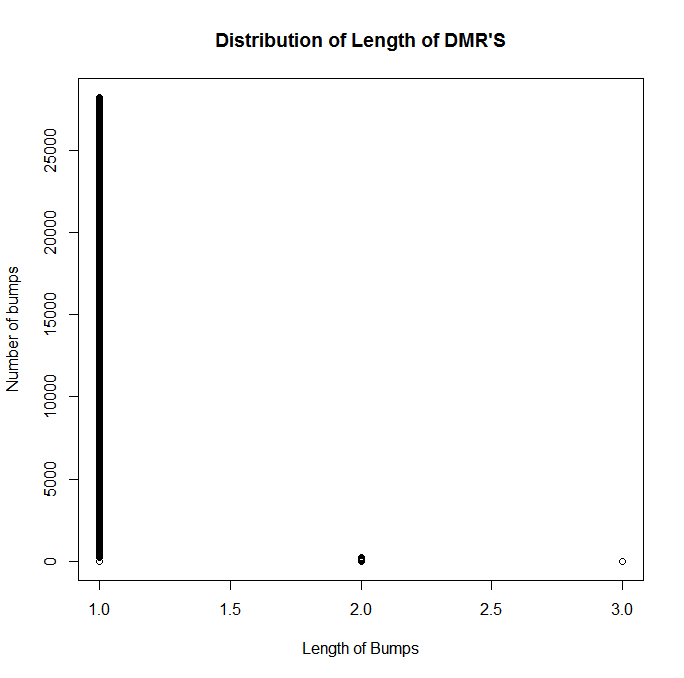
\includegraphics[scale=0.5]{bumpsDistribution.png}



\begin{verbatim}
Argument description for bumphunter,

cutoff: 

A numeric value. Values of the estimate of the genomic profile above the cutoff or
below the negative of the cutoff will be used as candidate regions. It is possible to
give two separate values (upper and lower bounds). If one value is given, the lower
bound is minus the value.

pickCutoff: 

Should bumphunter attempt to pick a cutoff using the permutation
distribution?

\end{verbatim}

\vspace{0.2in}

{\bf Analysis using Peaks files from DEVA}

This analysis uses the Peaks files generated from DEVA-v1.2, using the standard Nimblegen algorithms to identify peaks which coincide with methylated regions.

Sequential intersections, based on the number of peaks identified in each sample, was done in decreasing order for each experimental status. This step results in all the genes within each sample which are intersecting.

We find the common genes between “H460\_knocking” and “H460\_parent", and remove these genes from the intersected lists. We then order them by distance from the transcription start site(TSS).

{\tt NOTE:  Files are attached as “knockin\_genes\_distFromTSS.csv” and “parent\_genes\_distFromTSS.csv”. The distance is ordered in decreasing order of since the Max distance is a smaller positive number.}

The only features left in the result are transcription start sites, other possible feature is CpG Island (column name  is  FEATURE TRACK). The distribution of the distance from the TSS is also shown for both status types. The window for the Distance from the TSS is measured by  -5000 to +5000 , so window size is 10,000 bp (column name is SHORTEST\_DISTANCE\_FROM\_FEATURE\_TO\_DATA\_POINT).


{\bf H460\_knocking}

\begin{verbatim}

> table(annot_knock$FEATURE_TRACK)

transcription_start_site 
                     944 

> summary(annot_knock$SHORTEST_DISTANCE_FROM_FEATURE_TO_DATA_POINT)
   Min. 1st Qu.  Median    Mean 3rd Qu.    Max. 
-4998.0 -3363.0 -1916.0 -1956.0  -569.8   995.0 

\end{verbatim}•

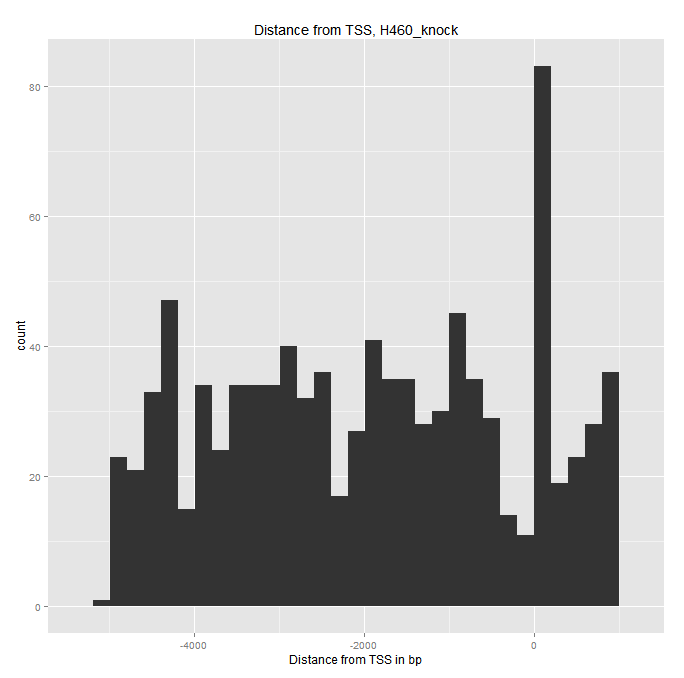
\includegraphics[scale=0.5]{distribution_knocking.png}


{\bf H460\_parent}

\begin{verbatim}

> table(annot_parent$FEATURE_TRACK)

transcription_start_site 
                     349 

> summary(annot_parent$SHORTEST_DISTANCE_FROM_FEATURE_TO_DATA_POINT)
   Min. 1st Qu.  Median    Mean 3rd Qu.    Max. 
  -4975   -3669   -2474   -2223    -718     997 

\end{verbatim}•

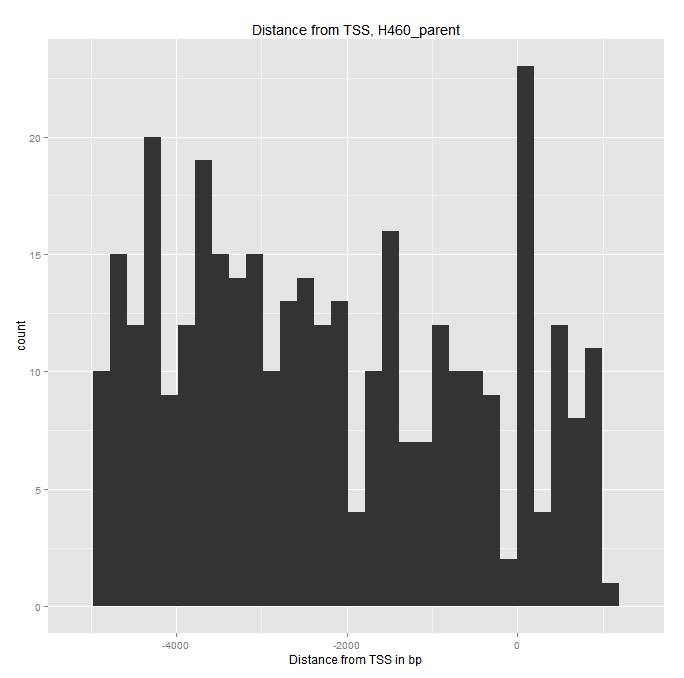
\includegraphics[scale=0.5]{distribution_parent.png}


%%%%%%%%%%%%%%%%%%%%%%%%%%
\section*{Algorithms and R-packages}
%%%%%%%%%%%%%%%%%%%%%%%%%%

List of R-packages used for analysis:
\begin{enumerate}

\item Charm

\item Bioconductor

\item BiocGenerics

\item RCircos

\end{enumerate}

Extracting the percentage methylation values from the raw data was done using {\tt charm::methp}, where the default arguments were used to normalize. The normalization methods included were spatial normalization(to correct for spatial artifacts), background subtraction(to estimate and remove the background signal before computing the log-ratios), loess within sample normalization and quantile between sample normalization.

These percentage methylation values are on a logit scale.

A regression based DMR-finding after correcting for batch effects pipeline was used in this analysis. Removing batch effects and using surrogate variables in finding DMRs ({\tt refer sva-package}) have been shown to reduce dependence on unknown noise in the data set.



%%%%%%%%%%%%%%%%%%%%%%%%%%
\section*{Comparisons}
%%%%%%%%%%%%%%%%%%%%%%%%%%



%%%%%%%%%%%%%%%%%%%%%%%%%%
\section*{Plots and Results}
%%%%%%%%%%%%%%%%%%%%%%%%%%

Circos plot was made using RCircos, the inner track refers to the H460 knocking genes and the outer track refers to the H460 Parent genes.

As it can be seen from the circos plot, very few chromosomes contribute to the methylated regions, including the sex chromosomes. The plot next to the gene names correspond to the peak values. It is easy to infer from this plot where there is a high frequency of methylated regions.

\includegraphics[scale = 0.3]{BiswalCircos4.png}



% %%%%%%%%%%%%%%%%%%%%%%%%%%%%%
% \section*{Future Possibilities}  
% %%%%%%%%%%%%%%%%%%%%%%%%%%%%%
% 
%The chromosome and locations obtained in the {\tt charm::dmrFind} function need to mapped to HG-19, to find corresponding genes. 
 
%Based on prior literature or studies we can determine which genes and regions show differential methylation and try to validate them with this study. 
% 
%Improvements have been made to the {\tt charm}-package's {\tt dmrFind} algorithm with a new package called {\tt bumphunter}, also included the Bioconductor repository for methylation analysis packages. {\tt bumphunter} acts as an adaptable package for finding peaks of methylation for experienced users. 
%
%{\bf NOTE:} Analysis of CHARM/MeDIP data through R-packages should be carefully done, using the correct genome builds. Support for HG-18 is being phased out, but there is a useful tool called {\tt rtracklayer}, available. This can be used to liftover your current regions to a more latest human genome build.
% 


%%%%%%%%%%%%%%%%%%%%%%%%%%
\section*{References}  
%%%%%%%%%%%%%%%%%%%%%%%%%%
\begin{enumerate}


	\item  Aryee MJ et al., Accurate genome-scale percentage DNA methylation estimates
	  from microarray data, Biostatistics (2011) 12(2): 197-210 	

	\item  Seth Falcon, Benilton Carvalho with contributions by Vince Carey, Matt
	  Settles and Kristof de Beuf. pdInfoBuilder: Platform Design Information
	  Package Builder. R package version 1.24.0.
	
	\item   Rafael A. Irizarry, Martin Aryee, Hector Corrada Bravo, Kasper D. Hansen and	Harris A. Jaffee (). bumphunter: Bump Hunter. R package version 1.0.0.
		
 \end{enumerate}

 
 
 
 
 \end{document}


